%%%%%%%%%%%%%%%%%%%%%%%%%%%%%%%%%%%%%%%%%
% Journal Article
% LaTeX Template
% Version 1.3 (9/9/13)
%
% This template has been downloaded from:
% http://www.LaTeXTemplates.com
%
% Original author:
% Frits Wenneker (http://www.howtotex.com)
%
% License:
% CC BY-NC-SA 3.0 (http://creativecommons.org/licenses/by-nc-sa/3.0/)
%
%%%%%%%%%%%%%%%%%%%%%%%%%%%%%%%%%%%%%%%%%`

%----------------------------------------------------------------------------------------
%	PACKAGES AND OTHER DOCUMENT CONFIGURATIONS
%----------------------------------------------------------------------------------------

\documentclass[twoside]{article}

\usepackage{lipsum} % Package to generate dummy text throughout this template

\usepackage[sc]{mathpazo} % Use the Palatino font
\usepackage[T1]{fontenc} % Use 8-bit encoding that has 256 glyphs
\linespread{1.05} % Line spacing - Palatino needs more space between lines
\usepackage{microtype} % Slightly tweak font spacing for aesthetics

\usepackage[hmarginratio=1:1,top=32mm,columnsep=20pt]{geometry} % Document margins
\usepackage{multicol} % Used for the two-column layout of the document
\usepackage[hang, small,labelfont=bf,up,textfont=it,up]{caption} % Custom captions under/above floats in tables or figures
\usepackage{booktabs} % Horizontal rules in tables
\usepackage{float} % Required for tables and figures in the multi-column environment - they need to be placed in specific locations with the [H] (e.g. \begin{table}[H])
\usepackage{hyperref} % For hyperlinks in the PDF

\usepackage{lettrine} % The lettrine is the first enlarged letter at the beginning of the text
\usepackage{paralist} % Used for the compactitem environment which makes bullet points with less space between them
\usepackage{graphicx} % Used for including images

\usepackage{abstract} % Allows abstract customization
\renewcommand{\abstractnamefont}{\normalfont\bfseries} % Set the "Abstract" text to bold
\renewcommand{\abstracttextfont}{\normalfont\small\itshape} % Set the abstract itself to small italic text

\usepackage{titlesec} % Allows customization of titles
\renewcommand\thesection{\Roman{section}} % Roman numerals for the sections
\renewcommand\thesubsection{\Roman{subsection}} % Roman numerals for subsections
\titleformat{\section}[block]{\large\scshape\centering}{\thesection.}{1em}{} % Change the look of the section titles
\titleformat{\subsection}[block]{\large}{\thesubsection.}{1em}{} % Change the look of the section titles
\bibliographystyle{plain}
\graphicspath{.}

\usepackage{fancyhdr} % Headers and footers
\pagestyle{fancy} % All pages have headers and footers
\fancyhead{} % Blank out the default header
\fancyfoot{} % Blank out the default footer
%----------------------------------------------------------------------------------------
%	TITLE SECTION
%----------------------------------------------------------------------------------------

\title{\vspace{-15mm}\fontsize{24pt}{10pt}\selectfont\textbf{Geoanalysis of the 2016 US Presidential Elections using Twitter Data}} % Article title

\author{
\large
\textsc{Saurabh Sood} \\
\normalsize University of Colorado Boulder \\ % Your institution
\normalsize \href{mailto:saurabh.sood@@colorado.edu}{saurabh.sood@colorado.edu} % Your email address
\vspace{-5mm}
}
\date{}

%----------------------------------------------------------------------------------------

\begin{document}

\maketitle % Insert title

\thispagestyle{fancy} % All pages have headers and footers

%----------------------------------------------------------------------------------------
%	ABSTRACT
%----------------------------------------------------------------------------------------

\begin{abstract}
This paper attempts to analyze the 2016 United States Presidential Elections from a geospatial perspective. Analysis is done on a collection of Geotagged tweets. The main purpose of the paper is to find out which agendas of the prospective candidates resonates with voters, which ones may negatively impact a candidates chances. As the collected tweets are geotagged, they are analyzed from a geospatial perspective, and the sentiment for the candidate is plotted on a choropleth map. One of the main observations from the analysis was, that most of the tweets carried negative sentiment, and that people generally rant on twitter, rather than discussing issues related to the election.
\end{abstract}

%----------------------------------------------------------------------------------------
%	ARTICLE CONTENTS
%----------------------------------------------------------------------------------------

\begin{multicols}{2} % Two-column layout throughout the main article text

\section{Introduction}

The analysis of the Presidential Elections in the United States is a challenging task, mainly due to the sheer number of factors involved. It is a hard job to statistically predict the outcome of the elections. Sentiment Analysis is one of the techniques which could be used to determine whether a candidate could win the election or not. The candidate's views on various topics, policies, and the sentiment associated with it could go a long way in determine whether a candidate would win or not.  \\

Twitter is a very important social network. What sets it apart from other social networks is the fact that Twitter data is public. It could be viewed by someone who doesn't have a Twitter account. The fact that a Twitter feed could be embedded in other pages is also a significant factor in Twitter being all pervasive in the social media space. \\

The tweets collected for the purpose of this paper are geotagged, which becomes possible to localize the sentiment in a particular area. For the purpose of this paper, the sentiment on various agendas of the candidates would be gauged based on the origin of the tweet. With this, the popularity of a particular candidate in a specific area/state will be determined. The paper focuses on the main presidential candidates in 2016, namely Hillary Clinton, Bernie Sanders, Donald Trump, and Ted Cruz. \\

There has been prior work in gauging public sentiment using Twitter. The work of Hao Wang et al\cite{Wang:2012:SRT:2390470.2390490} deals with large scale Twitter analysis for the 2012 presidential election. This paper attempts to build on that paper, and factor in the geospatial aspect by using geotagged tweets for the analysis.

\section{Data}
The data for the purpose of the paper is collected from the Streaming API of Twitter. The Streaming API of twitter provides an asynchronous long polling mechanism to retrieve tweets from the Twitter API. The advantage of the long polling is, that it does not hold the connected between the API server and the client. This enables the script to execute code only when tweets are made available. As the US presidential elections carries global interests, a lot of people not from the US could be tweeting about the candidates. To gauge the public sentiment in the US, it makes sense to restrict the tweets being analyzed to those from the US. For this purpose, the \textit{location} filter was applied in the calls made to the Twitter API, so that only tweets from the USA were retrieved from the API. The \textit{location} filter specifies a bounding box, which will be used to localize the tweets. A tuple of the Southwestern, and Northeast coordinates is needed by the Twitter API. The bounding box used for the purpose of this paper is [(-117.477, 32.496), (-67.2038, 44.6103)].

To retrieve the tweets from the API, the Tweepy\cite{Tweepy} library for Python was used. Tweepy provides a consistent access to the Twitter API, and includes OAuth authentication. A Drawback with the Twitter API is that it does not allow for multi-filtering. This means, that if the \textit{location} filter has been applied, then filtering for a particular hashtag, or text does not work. The workaround to this limitation is to filter for particular hashtag's in Python code. Once the geotagged tweets are retrieved, they are filtered for the keywords \textit{cruz}, \textit{clinton}, \textit{trump}, \textit{sanders}, \textit{bernie}. All the tweets pertaining to the presidential candidates are retrieved separately. \\

Twitter data is very unstructured. People tweet all sorts of stuff, such as links, images, sound clips, videos, and a lot of garbled text. This makes sentiment analysis and topic modelling challenging. In addition to the casual text, a lot of tweets are just retweets. A retweet is a repost of an original post. These also need to be handled properly, before further analysis could be done. For this purpose, before running the analysis, the tweets are preprocessed, so that only relevant text is used. For instance, URL's, images, mentions, usernames, are stripped out of the tweet.

\section{Methods}
Once the data has been collected and preprocessed, it is ready for analysis. The data consists of 7800 tweets collected for the presidential candidates. As an additional preprocessing step, all the tweets are combined into a single CSV(Comma Separated Values) file, and annotated with a tag, so as to identify that the tweet is for that presidential candidates. This will be required for analyzing sentiment for that presidential candidate. \\ \\
The system developed can be represented by the following block diagram: \\
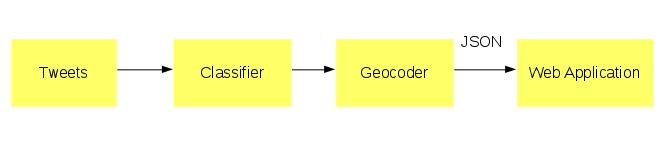
\includegraphics[width=1\columnwidth]{diagram}

\subsection{Sentiment Analysis}
For performing Sentiment Analysis, a Na\"{i}ve Bayes classifier\cite{naivebayes} is trained on a training corpus of 3200 tweets, equally divided among the presidential candidates is prepared. The remaining tweets are training data for the classifier. The training data is manually annotated as being positive or negative. \\
\textbf{Na\"{i}ve Bayes Classifier} \\
The Na\"{i}ve Bayes classifier is a bag of words classifier, which splits the data based on the word features. It is a conditional probability model. Given a set of $k$ classes, it computes the conditional probability of the given data belonging to all the classes, and returns the class with the highest conditional probability. Formally, this could be expressed by: \\
\begin{center}
$p(C_{k}|x_{1},x_{2}...x_{n})=\frac{1}{Z}p(C_{k})\prod_{i=1}^{n}p(x_{i}|C_{k})$
\end{center}  
where $C_{k}$ is one of $k$ classes, $x_{i}$ represent the set of word features, $Z$ is the scaling factor, $p(C_{k})$ is the class prior.\\
 
For the purpose of sentiment analysis of tweets, the tweet was divided into a set of words, and the conditional probability of it being in the positive and negative classes was calculated. The class it belongs to has the highest conditional probability. It is highly efficient for text classification.

\subsection{Web Application}
As the tweets are tagged by location, they can be geocoded to find out the coordinates required for plotting on a map. For geocoding, the Python \textit{geocoder} module \cite{geocoder} was used. Once the tweets are geocoded, the tweets are written to a JSON file, with the following structure: \\

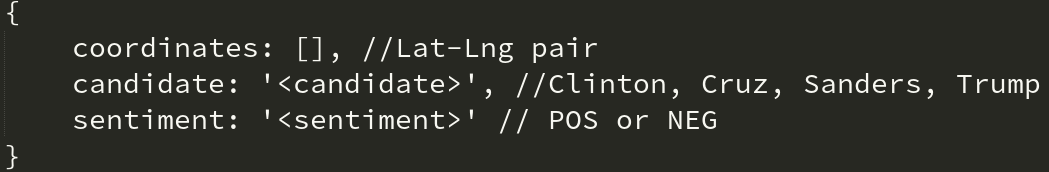
\includegraphics[width=1\columnwidth]{json}

A web application was created which reads the JSON\cite{json} file, and is used to plot points, representing the origin of the tweets on a map. The Google Maps API\cite{GMaps} was used to create the required tiles. The tweets are then aggregated by the State of Origin, and the percentage of negative tweets, and positive tweets was calculated using a Spreadsheet. The sentiment for the candidates was visualized using Datamaps\cite{datamaps}, which is a D3.js\cite{d3} library for creating maps.

\section{Results}

\subsection{General Observations}
While annotating the tweets for training the sentiment classifier, an interesting observation was made. Most of the tweets carried a negative sentiment. This could be attributed to the fact that there is a tendency to rant on a public social media platform. Supporters of a particular presidential candidate often target supporters of a rival candidate. There are frequent flame wars between supporters of rival candidates. This leads to a significantly large number of tweets carrying a negative sentiment. \\

On analyzing the tweets, another interesting observation was made with respect to the hashtags used. The hashtags are very consistently used by the supporters or detractors of the candidates. Some of the commonly used hashtags are \textit{\#ImWithHer}, \textit{\#NeverTrump}, \textit{\#FeelTheBern}.

\subsection{Sentiment Analysis Results}
On the test set of 6800 tweets, the Na\"ive Bayes algorithm gave an accuracy of 68\% with 5 folds cross validation. For the purpose of cross validation, 80\% of the training data was used for training, and the remaining 20\% of the training data was used as test data. \\
A major observation that was made in the classification was, that most of the tags were classified as negative. This could be explained by the fact that the majority of the training set comprised of negative tweets.

\subsection{Geovisualization}
A web application was created in Flask\cite{flask}. Flask is a framework for developing web applications quickly. The application exposes the following endpoints: \\
\begin{itemize}
\item
\textit{/} \\
This endpoint plots a Google Maps marker on a map, signifying the origin of a tweet. The HTML page provides option to select the candidate, and the sentiment, and the markers change corresponding to the candidate and sentiment selected.
\item
\textit{/<sentiment>/<candidate>} \\
This endpoint returns a JSON (JavaScript Object Notation) object for all the tweets of the specified candidate, and the specified sentiment
\item
\textit{/trumpchor} \\
This endpoint shows a choropleth map of the the sentiment for Donald Trump
\item
\textit{/clintonchor} \\
This endpoint shows a choropleth map of the the sentiment for Hillary Clinton
\item
\textit{/cruzchor} \\
This endpoint shows a choropleth map of the the sentiment for Ted Cruz
\item
\textit{/sanderschor} \\
This endpoint shows a choropleth map of the the sentiment for Bernie Sanders
\end{itemize}

The following Google Map showing all the tweets bearing Positive Sentiment for Hillary Clinton: \\ \\
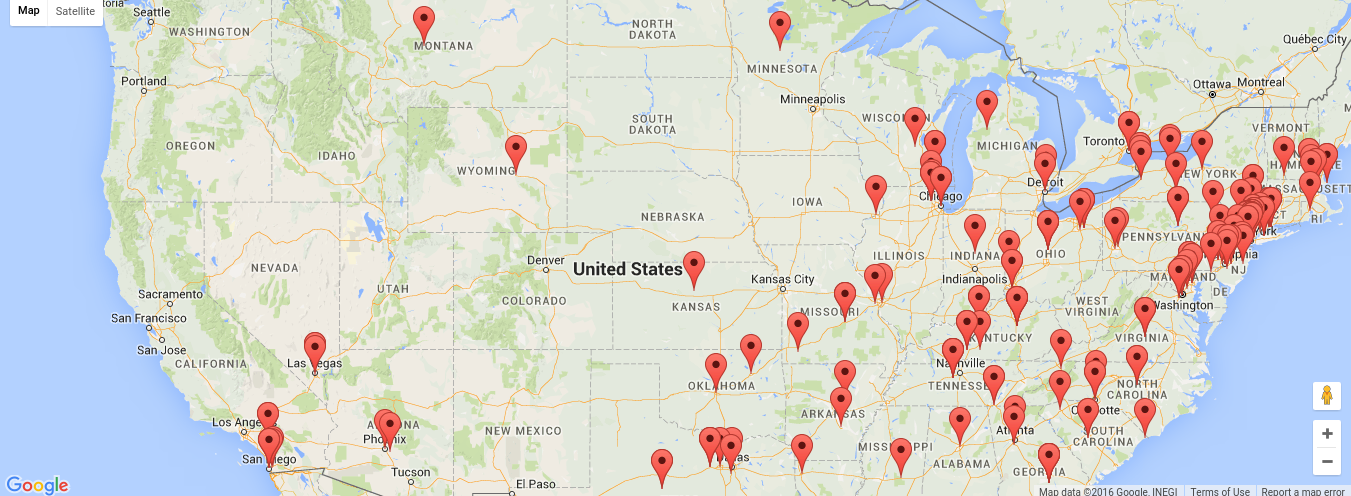
\includegraphics[width=0.95\columnwidth]{clinton-pos} \\ \\
The following Google Map showing all the tweets bearing Negative Sentiment for Hillary Clinton: \\ \\
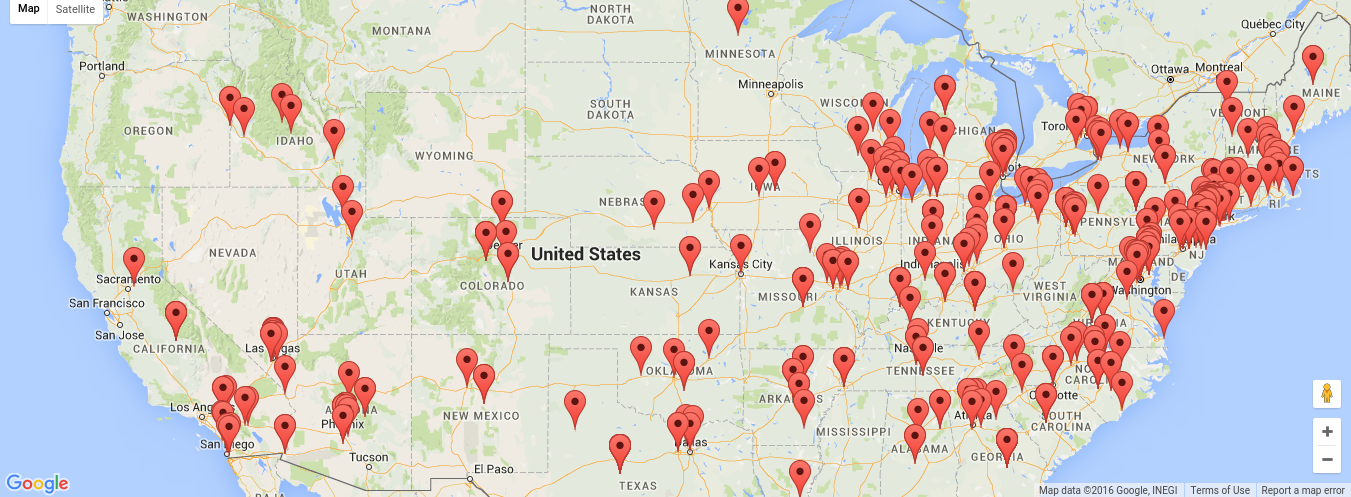
\includegraphics[width=0.95\columnwidth]{clinton-neg} \\ \\
The following Google Map showing all the tweets bearing Positive Sentiment for Bernie Sanders: \\ \\
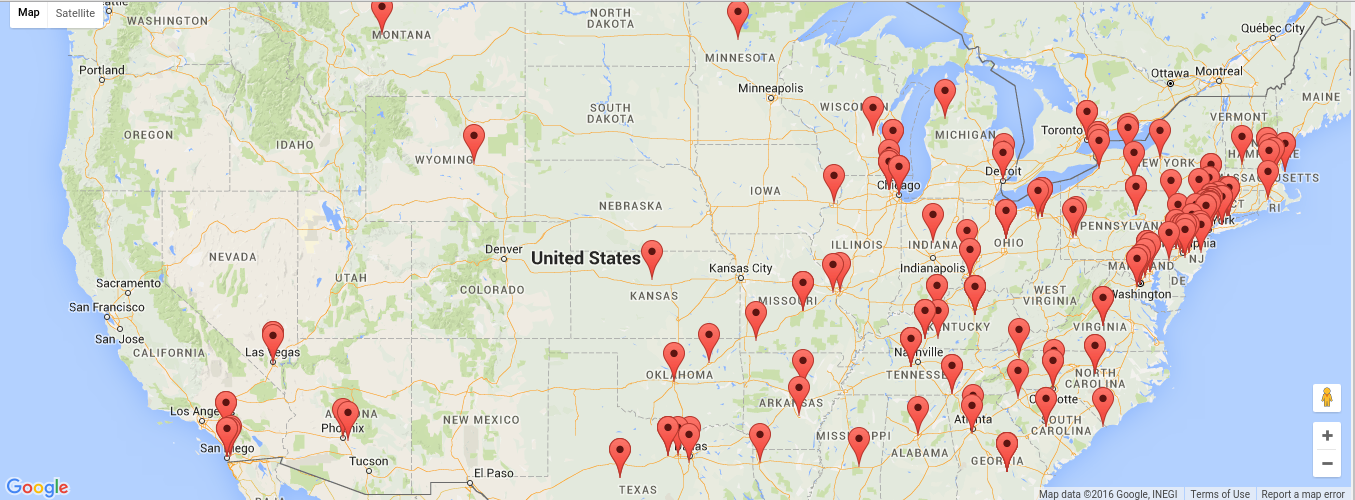
\includegraphics[width=0.95\columnwidth]{sanders-pos} \\ \\
The following Google Map showing all the tweets bearing Negative Sentiment for Bernie Sanders: \\ \\
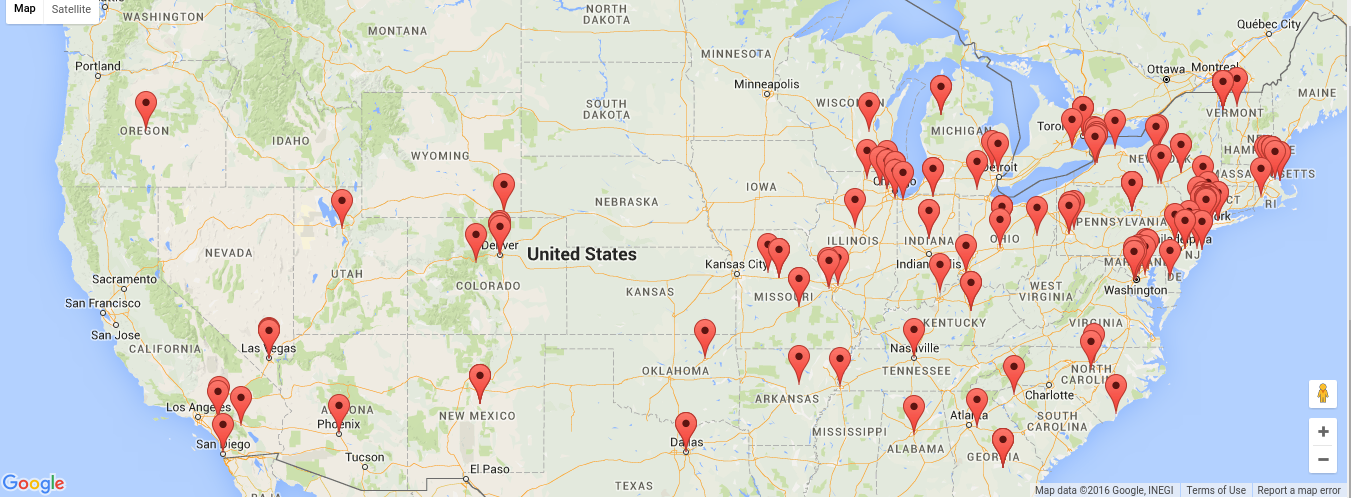
\includegraphics[width=0.95\columnwidth]{sanders-neg} \\ \\
The following Google Map showing all the tweets bearing Positive Sentiment for Ted Cruz: \\ \\
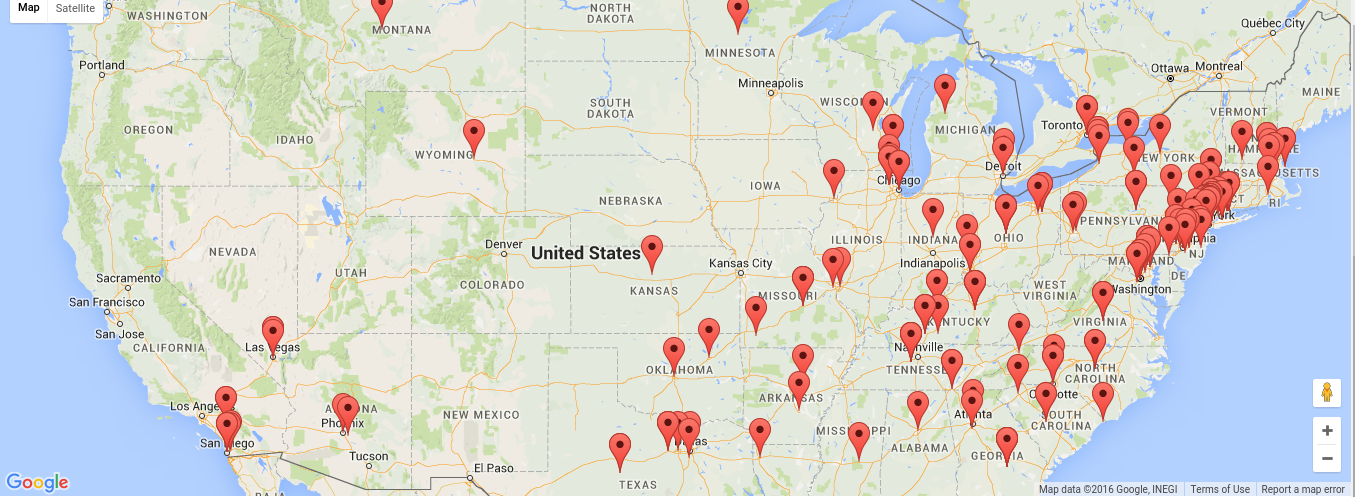
\includegraphics[width=0.95\columnwidth]{cruz-pos} \\ \\
The following Google Map showing all the tweets bearing Negative Sentiment for Ted Cruz: \\ \\
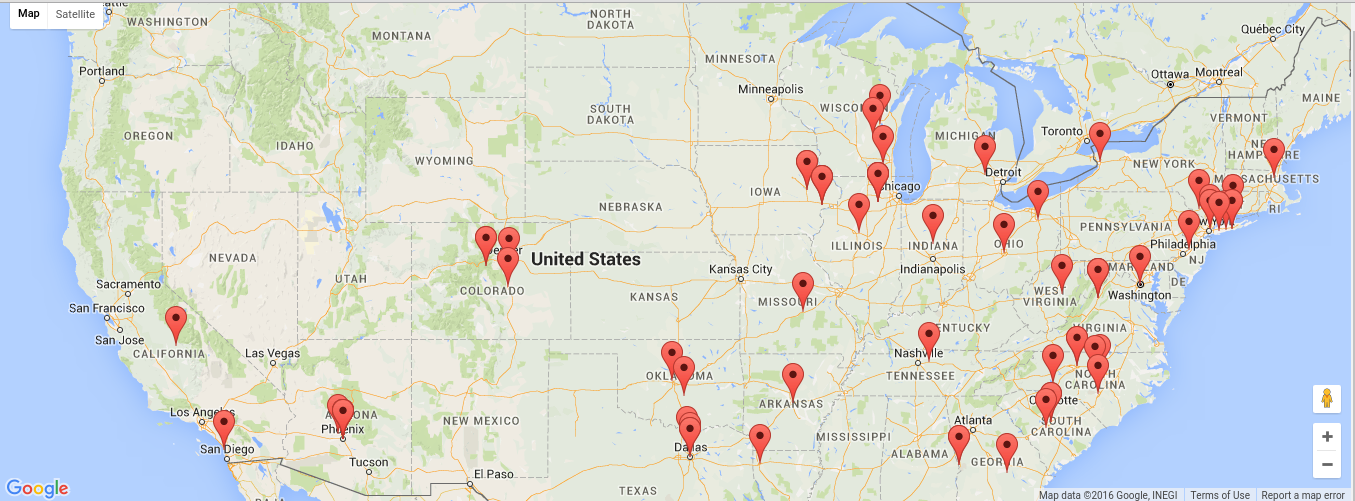
\includegraphics[width=0.95\columnwidth]{cruz-neg} \\ \\
The following Google Map showing all the tweets bearing Positive Sentiment for Donald Trump: \\ \\
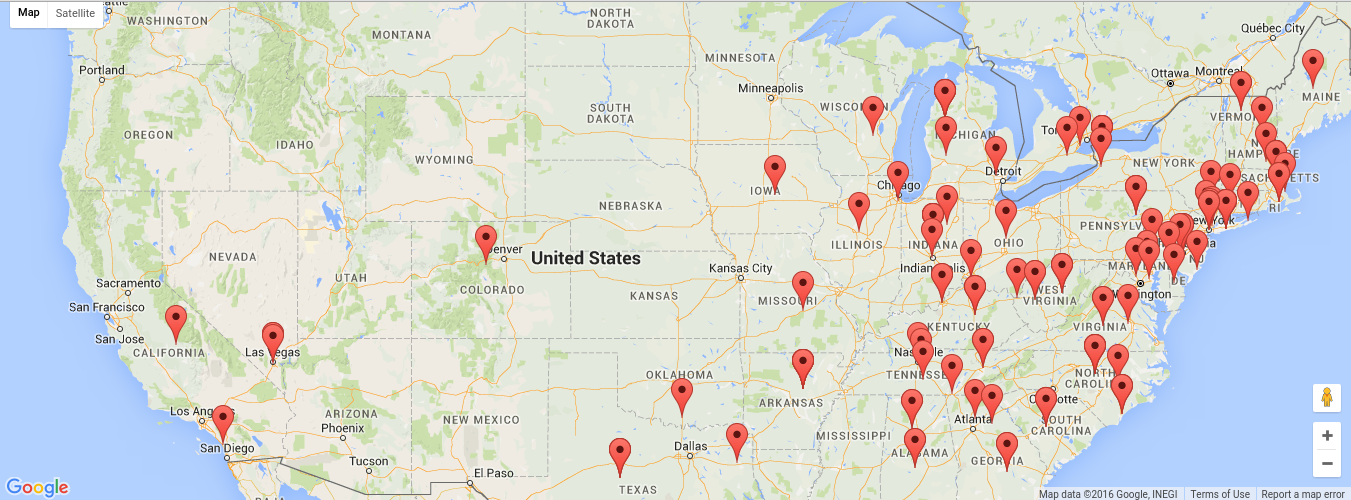
\includegraphics[width=0.95\columnwidth]{trump-pos} \\ \\
The following Google Map showing all the tweets bearing Negative Sentiment for Donald Trump: \\ \\
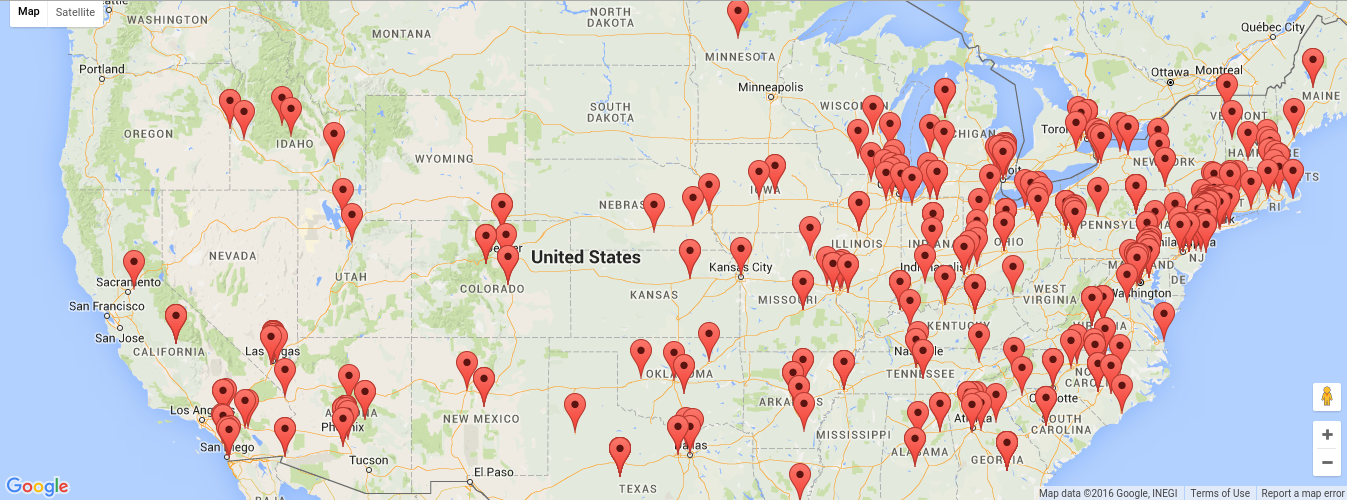
\includegraphics[width=0.95\columnwidth]{trump-neg} \\ \\

\textbf{Statewise Sentiment} \\
Once the tweets are geotagged, and a sentiment is attached to each tweet, they are grouped by the state of origin. Using a spreadsheet, the percentage of positive, and negative tweets is calculated for each candidate. This information is then used to plot a choropleth map, which shows the sentiment of each candidate in a particular state. \\

The following Choropleth map shows the statewise sentiment for Hillary Clinton: \\ \\
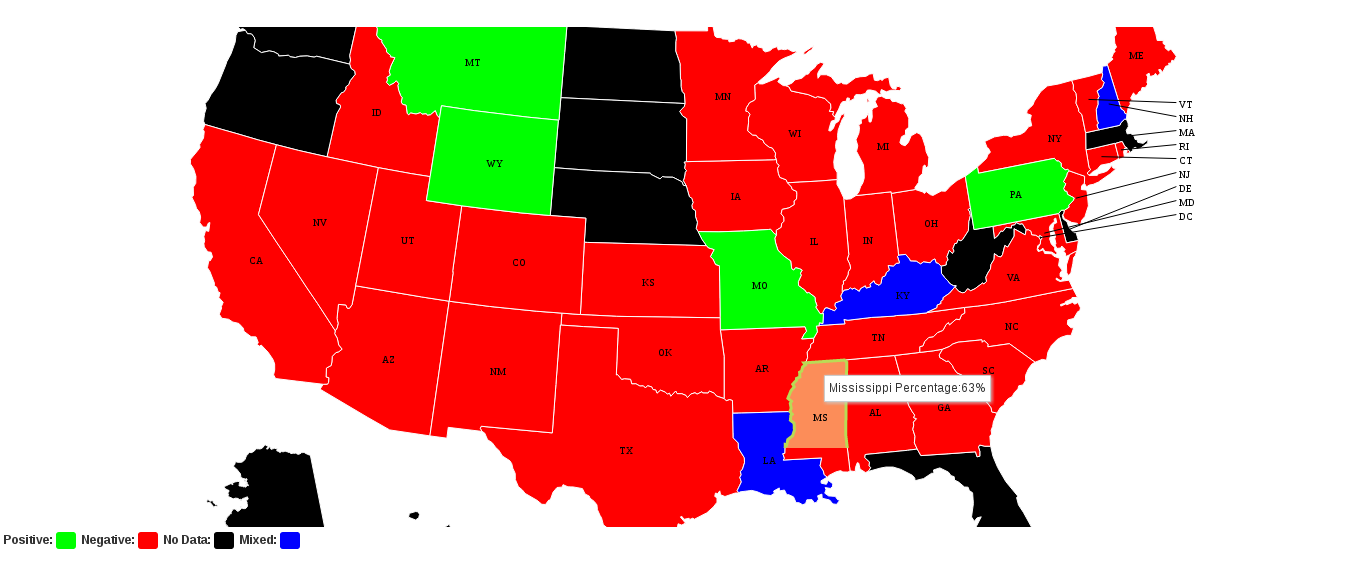
\includegraphics[width=1\columnwidth]{clinton-chor} \\ \\
The following Choropleth map shows the statewise sentiment for Bernie Sanders: \\ \\
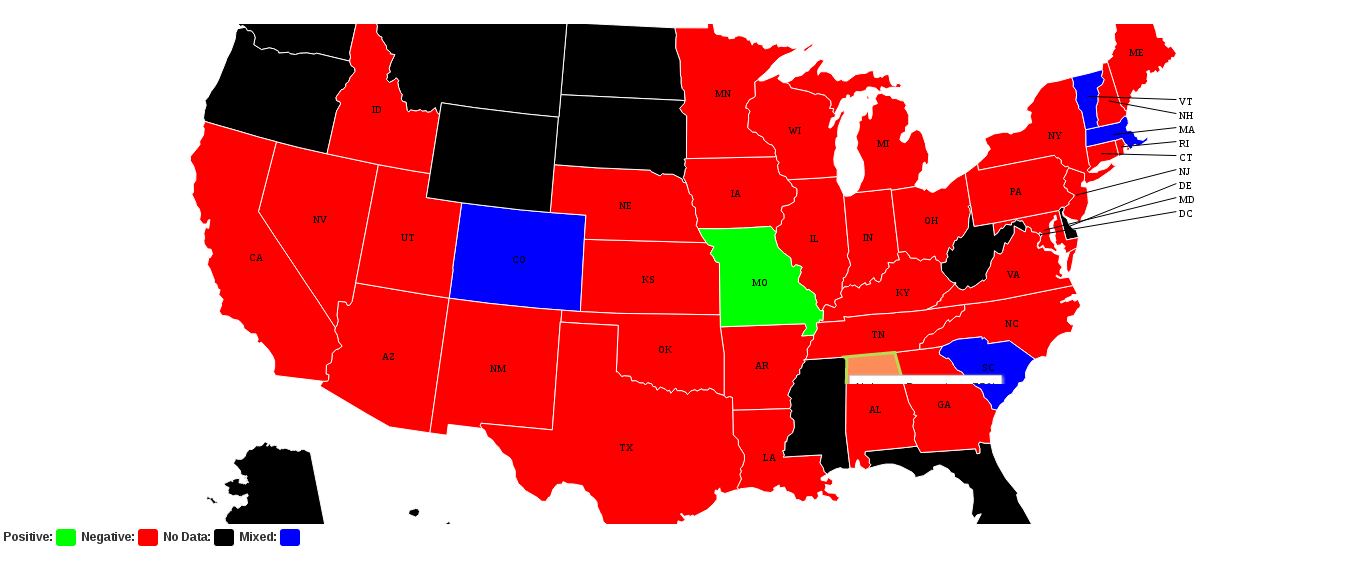
\includegraphics[width=1\columnwidth]{sanders-chor} \\ \\
The following Choropleth map shows the statewise sentiment for Ted Cruz: \\ \\
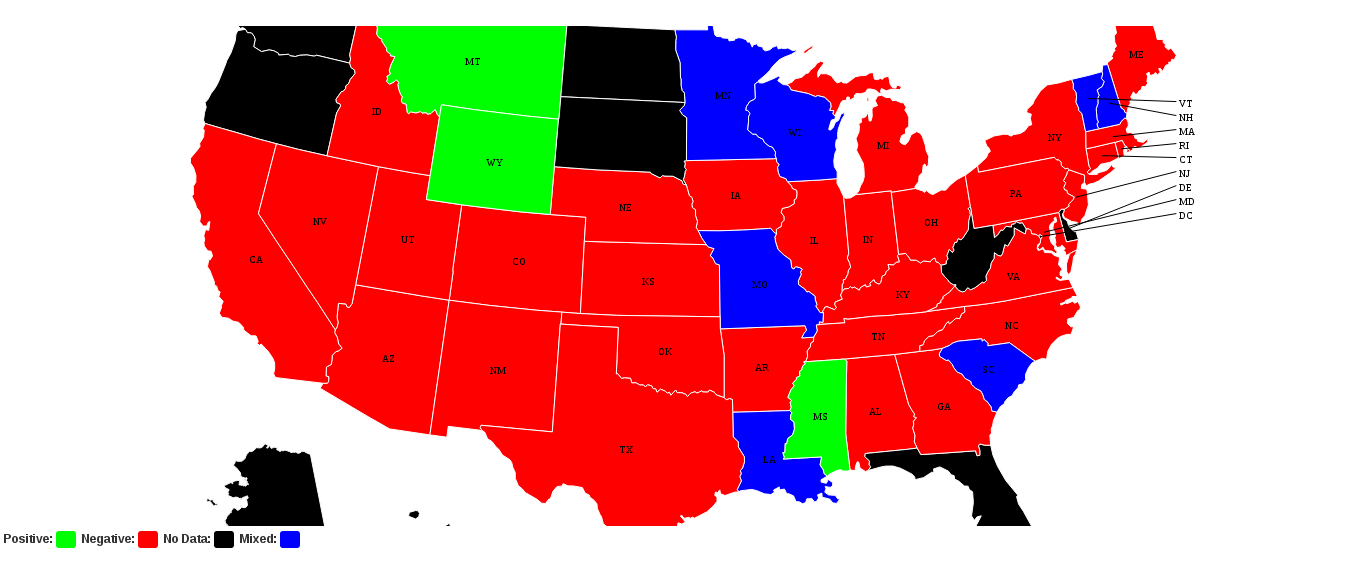
\includegraphics[width=1\columnwidth]{cruz-chor} \\ \\
The following Choropleth map shows the statewise sentiment for Donald Trump: \\ \\
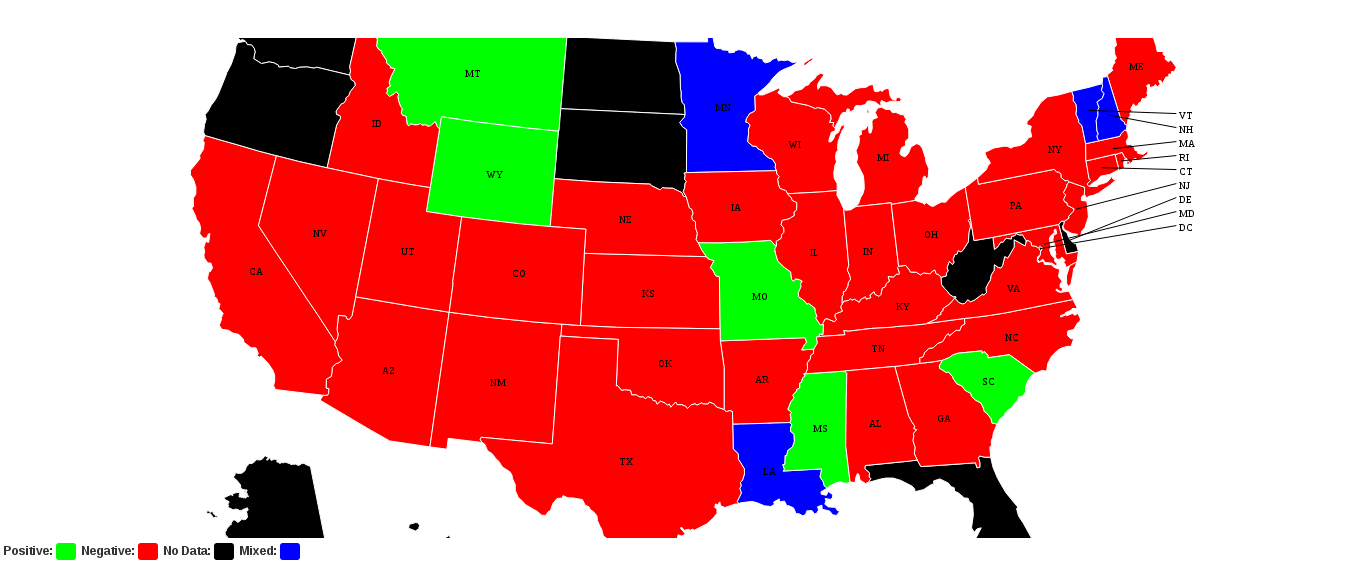
\includegraphics[width=1\columnwidth]{trump-chor} \\ \\

\textbf{Legend}
\begin{itemize}
\item Red: Negative
\item Green: Positive
\item Black: No Data
\item Blue: Mixed Sentiment (Equal number of positive tweets and negative tweets)
\end{itemize}

The choropleth maps throw some interesting observations: \\
\begin{itemize}
\item
Most of the states carry a negative sentiment for most of the candidates. This is to be expected, as the number of negative tweets far outweigh the number of positive tweets.
\item
The sentiment of Bernie Sanders is negative in most of the states. This is a little unexpected, as the number of positive tweets for Sanders is the highest for any candidate. The number of states for which Sanders has a positive sentiment is the least in comparison with all the other candidates.
\end{itemize}


\subsection{Sentiment on various topics}
While training the data, the sentiment for various topics for the particular candidate was observed and recorded, based on the content of the tweets. \\ \\
\textbf{Hillary Clinton}
\begin{itemize}
\item Negative on lying
\item Negative on the crime bill passed during Bill Clinton's presidency
\item Negative on the Email leaks
\item Negative on fracking
\item Negative on the Benghazi attack
\item Negative on corruption, and election funding
\item Negative on Surrogate Voting fraud
\item Negative on the Panama Papers
\item Mixed Sentiment on Black Lives Matter
\item Positive on Sexism
\item Positive on Gun Laws
\item Positive on Planned Parenthood
\end{itemize}

\textbf{Bernie Sanders}
\begin{itemize}
\item Negative on supporting the crime bill passed during Bill Clinton's presidency
\item Negative on Gun Laws
\item Negative on frequent attacks on Clinton
\end{itemize}

\textbf{Ted Cruz}
\begin{itemize}
\item Negative on 14 year citizenship requirement
\item Negative on stealing delegates in Colorado
\end{itemize}

\textbf{Donald Trump}
\begin{itemize}
\item Positive over losing Colorado delegates
\item Positive on being non establishment
\item Negative of not being informed about political process
\item Negative on racism
\item Negative on Lying
\item Negative on Corruption
\item Negative on running a negative campaign
\end{itemize}


\section{Conclusions}
The analysis of the US Presidential elections resulted in some interesting observations. A claim could be made that Twitter data is unreliable in predicting the outcome of an election, as most of the sentiment is negative. Also, people tend to rant on Twitter, leading to flame wars with supporters of rival candidates. However, Twitter is very effective in gauging the sentiment on various topics. \\

For the purpose of this paper, the sentiment on various topics was gauged by manually looking at the tweets, which were used for training the data. This could be done automatically by using a Topic Modeling algorithm, and then running sentiment analysis on the result. This is a good candidate for future work. \\

At this point, the paper doesn't deal with real time Twitter data. In the future, a system could be developed which would gather tweets in real time, perform the classification, recompute the sentiment for the state, and update the choropleth maps. 

\bibliography{main}
\end{multicols}
\end{document}
